\chapter{Introduction}
\label{chap:gf}

Magic has been a popular part of computer games since their beginning. In many games magic has its own lore and laws that make it systematical. Great examples of a complexity of magical spells are games \emph{Magicka} and \emph{Magicka 2}, where player casts spells by combining eight elements \ref{fig:magicka}. For example, using only earth element results in a rock thrown at the enemy, but adding fire will create a classic fireball.
\begin{figure}[!htb]
  \centering
  \label{fig:magicka}
    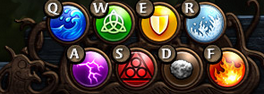
\includegraphics[width=0.5\textwidth]{ext/magicka.png}
    \caption{\emph{Magicka} spell interface}
\end{figure}

In books and movies, we can see wizards performing complicated hand gestures, or drawing on the floor some complex shapes. However, it is usually very easy to do magic in games, since players can cause magical storms by pushing few buttons. This spoils the feeling of magic as something extraordinary and secret. We would like to allow developers take a different approach, which requires players focus and concentration, as well as possible cooperation in spell casting.

While a majority of games binds spells to buttons, there are several games that used pattern recognition in their spell system. However, these systems recognized only simple gestures or patterns. Our goal is to make more robust recognition system, that allows players to draw complex patterns.

\section{Pattern recognition in current games}

Since symbols and gestures are an integral part of the magic, there were many attempts to bring them into video game environment. We can divide gestural system approaches into three categories, which are overlapping, as sometimes combination of these approaches can be used. The following categories and facts are taken from \cite{gameMagic}.

\subsection{Alternative controllers}
One such category are systems that utilize alternative controllers to mouse and keyboard, such as Kinect. Recent game representing this category is \emph{Fable: The Journey}, player casts spells by moving his hands, for example push spell is cast by pushing into the air. Kinect is used to track and recognize patterns made by the player. While moves are simple in nature, such as waving sideways or back and forth, both hands at the same time can be used, resulting in quite complex gestures.

\subsection{Restricted drawing forms}
Another technique used in several games is to let player draw into a predefined grid, or through predefined points. Both \emph{Castlevania: Dawn of Sorrow} and \emph{Deep Labyrinth} take advantage of Nintendo DS drawing interface that allows players draw magic signs. In \emph{Castlevania}, players draw signs by connecting glowing points in a circle in out of combat situations \ref{fig:castlevania}. \emph{Deep Labyrinth} introduces special casting interface as well, consisting of 3x3 sized grid, where player connects dots. These approaches take away part of the freedom, but they make recognition algorithms much easier, e.g. by tracing only the order of points and selecting the right spell.

\begin{figure}[!htb]
\begin{center}
\label{fig:castlevania}
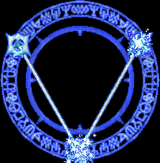
\includegraphics[width=.3\linewidth]{ext/castlevania.png}\quad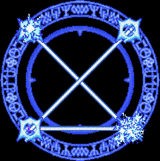
\includegraphics[width=.3\linewidth]{ext/castlevania2.png}
\end{center}
	\centering
	\caption{\emph{Castlevania: Dawn of Sorrow} spell interface}
\end{figure}

\subsection{Drawing}
Last category is for examples that are most similar to our goal. One of the first games to integrate some form of pattern recognition is \emph{Black \& White}, where player takes a role of the god. Using a mouse, players are able to cast miracles by drawing a specific pattern onto the ground \ref{fig:blackwhite}. Player can draw anything anywhere on the ground, and the game has to recognize if it matches some of the miracle patterns. Alternatively, they could also cast miracle by clicking on a button, possibly because a lot of players had trouble drawing the miracles. A similar approach to recognition of player drawn spells and their recognition was used in \emph{Arx Fatalis}. Players were drawing symbols into the air with a mouse, and the sequence of symbols represented some spell. While casting, game encoded mouse moves into characters in 8-directions precision, each direction representing some letter. After player finished their spell, a Levenshtein distance was calculated from each spell to the users created sequence and candidate with the lowest Levenshtein cost was returned as matching spell.

\begin{figure}[!htb]
\begin{center}
\label{fig:blackwhite}
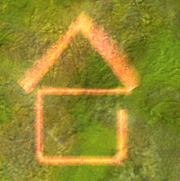
\includegraphics[width=.3\linewidth]{ext/gestureteleport.png}\quad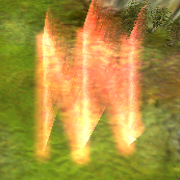
\includegraphics[width=.3\linewidth]{ext/gesturefireball.png}
\end{center}
	\centering
	\caption{\emph{Black \& White} teleport and fireball gestures}
\end{figure}

\section{Goals}

We would like to allow players draw complex spells. Instead of a sequence of symbols recorded over time, players could draw symbols arranged in a shape of another symbol, or embed one symbol in another. We also want our approach to be applicable in multi-player environments, where new situations can occur, such as multiple players drawing one spell. We don't want to introduce aiding structures such as trigger points, since they require order in which they were passed and force player to draw in a certain way or direction. They are also not very usable in a multi-player environment, since they can't handle multiple people drawing at the same time.

For the purpose of this work, we specify following requirements that we have on our recognition system.
TODO enumeration 

\subsection{Durability against shape deformations}
Since we want to recognize hand-drawn shapes, our system has to be prepared for human imprecise drawing, especially when drawing with a mouse. However, defining what is deformed within some boundaries and should be recognized, and what is too deformed, is not an easy task.

\subsection{Extendability}
We would like to offer easy-to-use library, that other developers can incorporate. For this purposes we would like to let them define their own shapes that should be recognized. Our framework will offer interfaces for both preparing their own shapes and using them in pattern recongition.

\subsection{Speed}
Our system should be applicable in demanding video games environment, prepared for the possibility of many players drawing their spells. To achieve this, we require fast recognition technique as well as usability in parallel environment. 

\subsection{Recognition of embedded shapes}
To allow players cast complex spells, we need to give them an ability to somehow encode multiple symbols in one spell. Theu might do is using shape embeddings. Each defined shape can contain several areas, where other shapes might occur. These areas and their content is then process in our recognition system as well.

\subsection{Recognition of shape conglomerations}
For the purpose of this work, shape conglomeration is a group of shapes representing the same shape class e.g. circle, arranged such that the whole conglomeration forms another shape. We can also look at it as taking the shapes lines, sampling many spots from them, and then replacing all the spots with the same shape.

\section{Approaches}

To achieve our goals, we divide the work into several steps. First, we will choose pattern recognition algorithm which best suits our needs from several reviewed algorithms. Then we modify it to recognize embedded shapes and shape conglomerations, since this topic is not very well covered. We use our system in simple game, but we try to utilize most of the abilities of our recognition system to demonstrate its functionality. Finally, we will measure its performance. We focus on two aspects of our implementation: speed and recognition effectiveness.

\chapter{Pattern Recognition}

\section{Pattern Recognition problem}
First, we need to define what we actually mean by pattern recognition. \begin{quotation}
The Pattern Recognition problem consists in determining a procedure that, on the basis of the attributes, excluding those that define the classification criterion assigns each entity to its proper class.
\end{quotation} \cite{formalMethods}
 Pattern recognition problem is a broad term for classification problems based on similarity of the features of classified objects, see \cite{formatMethods} for precise mathematical definition. We will focus more on the shape recognition problems category, which can be viewed as subcategory of pattern recognition. Shape can be typically defined as an equivalence class under the group of transformations, and the problem is then to algorithmically approximate the human-like visual pattern recognition. 

\section{Algorithms division}
There are hundreds of algorithms for pattern recognition as it is a central problem for computer vision. We divide pattern recognition algorithms by different properties.

We can divide them based on the creation process of the classifier into learning-based approaches and template-based approaches \cite{skeletonMatching}. In the learning-based approaches, pattern classifiers are obtained through training on classified samples. In the template based approaches, patterns are described by templates and the recognition problem transforms into searching for the best matching template for a given input image.

We can also divide the algorithms as stated in \cite{distanceTransform} based on the level of preprocessing into three classes: algorithms that use pixel values directly, e.g. correlation methods; algorithms that use low-level features such as edges and corners, e.g. distance transform method; and algorithms that use high-level features such as identified objects or relation between the features, e.g. graph-theoretic-methods.

\section{Normalized cross-correlation}
Following description is taken from the work of \cite{crossCorrLewis}.
Cross-correlation is a method to measure the similarity between a template and a given area of an image. The term cross correlation itself means a difference between two signals. Its one of the oldest approaches to pattern and feature recognition and extraction, and still serves as a base for more complex algorithms.
We compute an Euclidean distance of a image f and a template t, where pattern is on a position $(u\,v)$, by comparing corresponding pixels of the image at $(x\,y)$ and the template shifted to $(x-u\,y-v)$. 
\begin{equation*}
d_{f,t}^{2}(u,v)=\sum_{x,y} [ f(x,y) - t(x-u, y-v) ]^{2} 
\end{equation*}
When expanded, it gives us three terms. One of them is the cross correlation term $c(u,v)$.
\begin{equation*}
d_{f,t}^{2}(u,v)=\sum_{x,y} f(x,y)^{2} - 2c(u,v) + \sum_{x,y} t(x-u, y-v)^2
\end{equation*}
\begin{equation*}
c(u,v)=\sum_{x,y} f(x,y) * t(x-u, y-v).
\end{equation*}

Other two terms express energy (brightness) of template and image, respectively. We perform this computation for all possible values of u,v looking for the lowest value. Computing distance this way has several serious drawbacks. It is computationally heavy, it may give false matches if the image energy changes a lot with position. Also, range of values of cross correlation term depends on the size of the template and it is not invariant to scaling and rotation. 

The slowness of method can be partially solved by computing the cross correlation in a frequency domain using some form of a signal transform. Fourier transform is the common one, but other transformations were discovered, such as wavelet transforms [into.pdf p.90]. Convolution theorem states that when all conditions are met, Fourier transform of convolution is element-wise product of Fourier transforms of input signals. From Convolution theorem follows that time domain or space domain convolution is equivalent to element-wise multiplication in frequency domain. To compute convolution, we simply need to take element-wise multiplications of Fourier transforms of signals to be convoluted. Cross correlation differs in that we take the complex conjugate of the Fourier transform of the second signal.

Problems with range of cross correlation value and dependency on brightness can be fixed by using normalized cross correlation, where image and template vectors are normalized to unit length. Other desired aspects, such as scale invariance, has been addressed in many algorithms using cross correlation method. However, they usually introduce some trade-offs and they may not achieve all the required properties together. 

Normalized cross-correlation
\begin{equation*}
\gamma(u\,v) = \frac{\sum_{x\,y}f(x\,y) [f(x\,y)-\bar{f}_{u\,v}][t(x-u\,y-v)-\bar{t}]} {\{ \sum_{x\,y}f(x\,y) [f(x\,y)-\bar{f}_{u\,v}]^2 \sum_{x\,y}[t(x-u\,y-v)-\bar{t}]^2  \}^{0.5}}
\end{equation*}
where $\bar{t}$ is the mean of the feature and $\bar{f}_{u\,v}$ is the mean of $f(x\,y)$ in the region under the feature \cite{crossCorrLewis}.

\section{Shape matching and object recognition using shape contexts}
[TODO templateMatchingSimple.pdf ]
Shape matching using shape contexts is usually based on extracted features, which generally introduces more robust recognition of deformed images. In the reviewed algorithm, we try to find corresponding feature points of an image and a template, and we attempt to compute their distance as a sum of errors of corresponding points.

We treat an image as a set of points, and we assume that each shape is represented by a finite subset of its points. We extract from both image and template a certain number of feature points, the paper advises about 100 points. They need not to be key-points, such as maxima of curvature or corners. This allows us to use simple extraction method like edge detection. In our algorithm, we might also represent players drawings directly as a set of edges. 

With feature points extracted, we need to find corresponding points. To do so, in the [TODO templateMatchingSimple.pdf], they introduce shape context descriptor. For each sample point $p$, we can create a set of vectors originating from $p$ to all other feature points. Such set of vectors represents positions of other sample points relative to the origin point. The more sample points we choose, the more is this shape descriptor exact.

However, such descriptor might be too detailed and too sensitive to intraclass variations. In the paper, they presented more robust and compact shape descriptor. The idea is that for each point $p$, we compute coarse histogram by assigning other points to bins in polar coordinates with a center in $p$. [TODO polar coordinates image] Polar coordinates are more sensitive to points near p. We can then compute the cost of matching two pints as 

\begin{equation*}
C_{ij} =  C(p_{i}\,q_{j}) = \frac{1}{2} \sum_{k=1}^{K} \frac{(h_{i}(k) - h_{j}(k))^2}{h_{i}(k) + h_{j}(k)}
\end{equation*}

where $ h_{i}(k) $ and $ h_{j}(k) $ represent the K-bin normalized histogram at $p_{i}$ and $q_{j}$. Given a set of costs $C_{i,j}$ between all pairs of points $p_{i}$ and $q_{j}$, we need to find the best alignment, which means that we want to minimize the total cost of matching 
\begin{equation*}
H(pi) = \sum_{i} C(p_{i}\,q_{pi(i)}).
\end{equation*}
This can be solved in $O(N^3)$ time using the Hungarian method [templateMatchingSimple.pdf p5 ref 42]. 

We can achieve scaling invariance by normalizing all radial distances by the mean distance, and rotation invariance is obtained when searching for the lowest cost among all permutations. according to the paper, this method is robust against small geometric disturbances.

\section{Matching of Shapes Using Dynamic Programming}
Another method proposed by [DynamicProgramming.pdf] introduces an algorithm  which uses dynamic programming combined with high-level features. Similarly to the previous algorithm, we try to compute a distance of template and image, but in a different way.

The algorithm requires that both shape and template are represented as a sequence of convex and concave segments, split by inflex points. The idea of the algorithm is to recursively merge segments using two grammar rules $CVC -> C$ and $VCV -> V$, where V denotes concave and C convex segment. Simultaneously, merging cost is computed using a merging cost function, and results are stored into dynamic programming table, with additional information.

Rows and columns of dynamic programming table represent inflex points of shape and template, respectively. At the end of the computation, each field $F(i,j)$ contains the minimal cost of merging first i-1 segments of shape and j-1 segments of template. Minimum cost is computed as:

\begin{equation*}
g(i_{w},j_{w}) = min\{g(i_{w},j_{w}) + \phi(a(i_{w-1}|i_{w}), b(j_{w-1}|j_{w}))\}
\end{equation*}
where the minimum is over all possible values of 
\begin{equation*}
(i_{w-1}\,j_{w-1})  =  (i_{w} - 2m_{w} -1\, j_{w} - 2n_{w} - 1)
\end{equation*}
, where $m \geq 0$ and $n \leq 0$.
Since merging of convex and concave segments is not possible, merging always involves an odd number of segments. Dissimilarity cost function: 
\begin{equation*}
\phi(a(i_{w-1}|i_{w}), b(j_{w-1}|j_{w}))  =  \lambda MergingCost(a(i_{w-1}|i_{w}))  +
\end{equation*}
\begin{equation*} 
\lambda MergingCost(b(j_{w-1}|j_{w}))  +  DissimilarityCost(a(i_{w-1}|i_{w}), b(j_{w-1}|j_{w}))
\end{equation*}

where lambda value controls merging tendency. With lower value, merging is more encouraged. For shapes with much detail, it is practical to set higher values, otherwise, these details may be lost during merging. 

Since algorithm assumes, that first segments of shape and template are aligned and match, we may need to run the algorithm for all possible starting points of shape if we don't know the first segment beforehand.

Contrary to the previous algorithm, we now require extraction of high-level features, we need to extract convex and concave segments in correct order. However, we obtain a matching algorithm that is independent of shape translation, scaling and rotation. We can also directly control invariance to deformations using lambda parameter.

\chapter{Neural networks}
Neural networks are mathematical models inspired by a behavior of a biological nervous system. They have been successfully used to solve problems in many different areas, including image and pattern recognition. They can be used in problems, where we can't mathematically describe the solution given the instance of the problem, or doing so would be overly complicated. We have chosen neural networks approach as a core of our system. They don't require feature extraction, since they can learn it themselves. They also have a great ability to generalize, which has been useful for recognition of shape conglomerations.

\section{Neuron}
Artificial neural networks are structures built for parallel data processing. The basic network unit is a neuron, which is characterized by its input and output connection weights, the activation function and bias.

TODO model of neuron obrazek
TODO activation function

\section{Artificial neural network}
Artificial neural network is a mathematical model, consisting of a set of neurons interconnected by connections.
More exactly it is a set 
$
M  =  (N,C,I,O,w,t), where: $
 $N is a finite set of neurons,$
 $C \subset N x N is nonempty set of oriented connections,$
$I \subset N is nonempty set of input neurons,$
$O \subset N is nonempty set of output neurons,$
$w : C -> R is weight function, $
$t : N->R bias function.$

In practice, multilayer neural networks are commonly used. Multilayer networks are networks, in which neurons are organized in layers starting with input layer and ending with output layer, with hidden layers in between. For each neuron in this structure, its input connections originate only in a previous layer, and its output connections reach only to a following layer. 

\section{Learning process}
Learning process of an neural network is an optimization problem, where we want to optimize the error function. Error function describes a difference between actual and correct output values for given set of training data. One of the popular error functions is mean square error function:
\begin{equation*}
MSE  =  \frac{1}{n} \sum_{i=1}^{n} (Y_{i} - \hat{Y}_{i})^2.
\end{equation*}

Learning process consists of showing inputs to the network and adjusting its connection weights based on the actual and correct output values in order to lower the MSE.

\section{Learning algorithms}

\subsection{Back-propagation algorithm}
Back-propagation is one of the most popular algorithms for neural networks training, and it serves as a base for many other algorithms.

The algorithm is based on the gradient descent method. In the first step, input is evaluated and mean square error of output is computed. However, different error function may be used. Then we can apply chain rule for partial derivatives to get:
\begin{equation*}
\frac{\partial E}{\partial w_{ij}} = \frac{\partial E}{\partial a_{j}} \frac{\partial a_{j}}{\partial w_{ij}}
\end{equation*}

When we use sigmoid activation function, we obtain:
\begin{equation*}
\sigma_{j}  =  f'(a_{j})(d_{j} - y_{j}) = (1-y_{j})y_{j}(d_{j}-y_{j})\,
\end{equation*}
where $\sigma$ is weight change. This expression tells us, in which direction does the error function descent fastest.

Then we can evaluate the derivatives the error function like this
\begin{equation*}
\sigma_{j} = y_{j}(1-y_{j}) \sum_{k=1}^{c} w_{kj} \sigma_{k}
\end{equation*}
where the sum runs over all output units. Now we can update the weights with a formula for the output layer
\begin{equation*}
\Delta w_{ji} = - \eta \sigma_{j} x_{i}
\end{equation*}
and for hidden layers
\begin{equation*}
\Delta w_{ji} =  - \eta \sum_{n} \sigma_{j}^{n} x_{i}^{n}
\end{equation*}

In summary, the input is evaluated and difference between correct and actual output is computed using error function. The difference is propagated back through the network and weights are updated using the gradient descent method. The whole process is repeated until a desired error value is achieved.

\subsection{Quick-prop algorithm}
Algorithm is an improved version of back propagation. It is based on independent optimalization steps for each weight, rather than updating all weights at once. For the update computation, it requires data from the last iteration, which increases space complexity. 

\begin{equation*}
\Delta ^{(k)} w_{ij} = \Delta^{(k-1)} w_{ij}*(\frac {\bigtriangledown_{ij} E^{(k)})} {\bigtriangledown_{ij} E^{(k-1)} - \bigtriangledown_{ij} E^(k-1) - \bigtriangledown_{ij} E^{(k)} }
\end{equation*}
where $\Delta ^{(k)} w_{ij}$ is weight delta from \emph{kth} iteration and $\bigtriangledown_{ij} E^(k)$ denotes partial $w_ij$-derivation of error function E in kth iteration.

\section{Convolution neural networks}
Convolution neural networks are modern solution to image recognition. They are similar to classic neural networks, but the main difference is that they expect the input to be image, and they allow us to encode some of the properties of images naturally into their architecture.

Neurons of convolutional networks have a layered architecture, like classic networks, but their layers consist of neurons arranged in grid, just like pixels of an image, and each neuron is connected only to a small corresponding area in next layer.  
TODO image
\chapter{Implementation}
Implementation of the recognition system consists of two parts, one responsible for the actual recognition, and one for training of neural network based on user-defined shapes. The usage of the framework consists of three steps: TODO enumeration
1. defining the shapes and setting up desired recognition parameters.
2. training the neural network based using the defined shapes
3. using the framework and trained network to recognize patterns

\section{Data representations}

\subsection{Input image data format}
First, we have to define the form of input. There are two general approaches to representation of graphic data: vector graphics and raster graphics. Vector graphics data are usually more flexible, allowing us to perform deformations and scaling without loss of precision. They also take less space and can be converted into pixel map when needed. On the other hand, they are harder to produce, since because they are built on the knowledge of mathematical relations in the image. Since we expect the input to the program to represent rather simple black and white shapes or their combinations, without any additional information like color or different shades, we have decided to create the interface for vector graphics like input.

\subsubsection{Image lines class}
Input to the shape recognition program is in the format of instance of \emph{ImageLines} class, defined in \emph{ImageAnalyzer.h} header file. This class wraps a vector of lines defining the shape, accessible through \emph{GetImageLines} method. The user is expected to fill the vector with lines representing the two dimensional image before passing it into the \emph{Analyze} method. The class offers several other methods, used primarily by the recognition algorithm. 
Line is represented by the instance of class \emph{Line} in the same file, and the constructor accepts two \emph{float2} type vectors, first containing the start coordinates of the line, and second containing the end coordinates. Internally, the coordinates are transformed into three dimensional vectors into homogeneous coordinate system. 

\subsection{Shape descriptors}
Shape descriptors are key part of the system, as they are used during training of the neural network to produce shape examples and during analysis of image they provide the algorithm with information about the expected line positions and possible embedded shape locations. User can define their own shapes by inheriting from abstract class \emph{ShapeDescriptor} defined in \emph{ImageAnalyzer.h} file. The core of shape description using this class are parametric curves. Abstract class functions, which should be defined by user, take parameter \emph{t} in range $[0-1]$ as an argument, and return a point on the curve in a 2D space in a range $[0-1]^2$. The curve does not have to be continuous, but it has to return value for every parameter value in the range, and also thread safety of some methods is required. It is recommended to keep the shape complexity low, as some very small details may be lost in the data preparation for the training. 

\subsection{Output data format}
Output is in the form of instance of \emph{ShapeNode} class defined in \emph{ImageAnalyzer.h} file. It represents a tree structure, where each node contains the recognized shape index, conglomeration shape index and embedded shapes as children.

\section{Recognition process}
The recognition process starts in the \emph{Analyze} method, declared in \emph{ImageAnalyzer.h} file. It accepts an instance of \emph{ImageLines} class as an argument, and returns \emph{ShapeNode} instance describing the recognized elements in the image. The image lines are first normalized, which means transformed into $[0-1]^2$ coordinate space. This transformation is essentially a rescaling, preserving the length ratio and angles. Then, the top level shape is analyzed by drawing the lines into pixel map passing the pixels into the trained neural network. If rotation recognition is enabled, the image lines are rotated several times by a fixed angle value, and then drawn and analyzed by the network again. The network return a vector of values, each value representing the similarity to the shape it represents, and the highest value shows the matched shape. If there are more network outputs for different rotations, the first highest value among all outputs is considered. If the highest value is not greater than certain fixed value, shape is not recognized. Recognized shape is returned along with its matching rotation, in which it scored the highest similarity.

\subsection{Compound shape}
When the top level shape is recognized, its shape descriptor is used to sample the theoretical curve points uniformly on the range of \emph{t} on interval $[0-1]$. Then, for each sampled point, this point is expanded into small square, the original image is clipped to this square, discarding the lines outside, and the result is analyzed for for any recognizable shape. Recognized shapes are counted over all samples, and if the count of any shape is high enough, the top level shape is recognized as a compound shape created from a number of smaller shapes of the type with the highest count. Shapes, that form the composition are not tested for compound shape again to optimize the speed and because creating such recursion of compound shapes is unexpected.

\subsection{Embedded shape}
To recognize embedded shapes, we use the shape descriptor of the shape recognized previously, and focus on the embedded shapes locations. For each embedded shape location defined in the shape descriptor, we clip the image lines to that area, and recursively run the \emph{Analyze} method on the result.

\section{Neural network preparation}
We use the \emph{FANN} neural network library to train and use neural networks. This open source software is easy to use and install, while having a lot of options in terms of network architecture and training. Thanks to its simplicity, we were able to develop an automatized training system for the networks.

\subsection{Data generation}
Training a neural network that is able to recognize user defined shapes requires training data. We generate the training data based on the shape descriptors registered by user. To generate a data sample for neural network, we take the shape descriptor, and create an \emph{ImageLines} instance from it. It will be either deformed simple shape instance, or instance of compound shape. In the case of creating deformed simple shape instance, shape curve is sampled many times using the shape descriptor, and each sample can be moved in the direction perpendicular to the line between the original position of the last point, and the original position of this point. TODO picture. This offset is linearly magnified and then reduced, resulting in a heuristics that tries to approximate some of the human like deformations of drawn shapes. Then, line between previous and new point is added to the image instance. In the case of the shape conglomeration, the shape curve is sampled much less frequently and each point is replaced by rescaled image lines of a randomly chosen shape, but this shape is the same for the whole composition.

\subsection{Training}
Training is done using the generated data from the previous methods and the \emph{FANN} library. First, the training data and test data are generated, where the size of training data can be changed by the user, and the size of test data is one third of the size of training data. Then the network is repeatedly trained on the training data until it reaches the user set up MSE, or until it stops improving. Internally, it starts with high MSE target value, which is then gradually lowered, and in between the improvement ratio is checked. The algorithm used for training the network is called \emph{RPROP}, an improved version of quickprop algorithm, because we achieved best results with this algorithm in terms of the improvements stability. In the neural network, we use an \emph{Elliot} activation function.

\section{Game prototype}
The game, which demonstrates the usage of this pattern recognition work, has been developed using URHO3D game engine in version 1.7. \begin{quotation} Urho3D is a free lightweight, cross-platform 2D and 3D game engine implemented in C++ and released under the MIT license. Greatly inspired by OGRE and Horde3D. \end{quotation} It is easy to learn and use, and comes with many examples together with source codes of how to use it. It is built on a component based scene model. 

\subsection{Game description}
TODO

\subsection{Spell system}
The game spell system consists of several parts. First is the \emph{DrawableTexture} component, which is attached to the ground entity. This component is able to track players drawings and store them as an lists of points, each list representing one continuous line. When the player presses the button to cast spell, the \emph{Caster} component attached to their character extracts the lines in rectangular area around the character and transforms them into the vector of lines. Then the instance of \emph{Spell} class defined in \emph{SpellSystem.h} file is created. There, the \emph{ImageAnalyzer::Analyze} method is finally called in a different thread and when the analysis is done, the result is parsed and the spell is casted.

\chapter{User guide}
\section{Recognition system}
\subsection{Creation of shape descriptor}
For the training as well as for the recognition, shape descriptors are required. The shape descriptors have several behavioral limitations, that need to be followed by the user. The intended purpose of the descriptor is to describe a single 2D shape in a $[0\,1]^2$ rectangular area. The descriptor is expected to return the same shape every time, without any modifications, and all of its methods should return the same values when called with the same parameters. It is also required, that all of the shape descriptor methods are thread safe. It is then recommended to design the shape descriptor as a class with constant inner state. Not following these rules may result in unexpected and dysfunctional behavior of the system. User can create a shape descriptor by including the \emph{ImageAnalyzer.h} header file, and inheriting from the class \emph{ShapeDescriptor}. This class contains several abstract methods, that should be implemented:
\begin{enumerate}
\item [GetName] Method, that returns the name of the shape a string. This is only for debugging purposes and it does not have to be unique or even constant. However, it is recommended to return a constant unique name among the descriptors.

\item [GetPoint] Function overload with one parameter \emph{t} returns a point of the curve, based on the \emph{t} parameter. It is recommended to normalize the parameter into $[0\,1]$ range by \emph{NormalizeParam} function.

\item [GetPoint] Function overload with three parameters, that allows the descriptor to describe noncontinuous curves. The \emph{point} parameter passed by reference should be filled with the value of \emph{GetPoint(t)} as it describes the point of the curve. Then the function should return true, if the curve is continuous on the interval $[last_t\, t]$, otherwise false.

\item [GetPointsOfInterest] Function, that describes a places, where an embedded shape may appear. It returns a vector of \emph{float3} type, where the first two numbers denote the top left corner of the square area, and the third number is the size of the square.
\end{enumerate}

Examples of shapes descriptors can be found in the \emph{ExampleShapeDescriptors.h} file.

\subsection{Algorithm properties}
There are several variables then can be set up and influence the functionality of the software. They can be found in the \emph{ImageAnalyzer} namespace. Some of them are used both in the training and in the recognition. It is necessary then for the user to be consistent and use the same settings for the recognition as they used for the training.

\begin{enumerate}
\item [DEBUG\_IMAGE\_SAVE] Boolean variable with default value false. If true, the images created during the recognition are saved as BMP files onto the hard disk, but only in the initial rotation of the image.

\item [COMPOSED\_SHAPES\_ENABLED] Boolean variable with default value true. If false, recognition algorithm recognizes the whole shape, but does not search for the smaller shape that might compose it. During training, the examples generating algorithm does not produce compositions of shape, so the network is not trained to recognize the shape of the composition.

\item [EMBEDDED\_SHAPES\_ENABLED] Boolean variable with default value true. If false, recognition algorithm ignores the positions, where embedded shapes might be, and recognizes only the top level shape and its composing shape. During training, the generating algorithm will not generate embedded shapes, and the network will not be trained to filter out these locations, where they might appear.

\item [ROTATIONS\_ENABLED] Boolean variable with default value true. If false, recognition algorithm will not test different shape rotations for the best match, but will rather use the initial rotation. This variable does not have impact on training, since rotation recognition is not a task of the neural network.

\item [DEBUG\_OUPUT] Integer variable with default value 1. Controls the amount of debug info of the recognition system. If set to 0 or lower, no debug output is produced. If set to value 1, prints recognized shape with its matching rotation and its composing shape, for the top level shape and each embedded shape. If set to 2 or higher, produces the same output as with value 1, but also all network outputs from the analysis are printed for all the rotations.

\item [IMAGE\_SIDE\_SIZE] Integer variable, controls the size of the images that are created during analysis. Every time there is an instance of \emph{ImageLines} class that should be analyzed by the network, the lines are drawn into the square pixel map of size set by this variable. It is also directly connected with the network input layer size, which has to be a second power of this value. The default value is 32, which means that the neural network has an input layer of size 1024 neurons, and the images produced in the algorithm are pixel maps of $32*32$ pixels.

\end{enumerate}

\subsection{Training phase}
Training the neural network consists of several steps. First step is to set up the variables controlling the behavior of the recognition and training algorithms. By including the \emph{Training.h} file, user can access the \emph{ImageAnalyzer} namespace for setting up the variables, and the \emph{Training} namespace for the training functions. After setting the variables, it is necessary to register the desired shape descriptors through function \emph{Training::RegisterShapeDescriptor}. This function takes a unique pointer to shape descriptor as its parameter, and returns an instance of \emph{ShapeIndex} class. This class is only a wrapper over integers but it works as an identifier of the shape for the network. Then it is necessary to create an instance of \emph{TrainingCase} class, representing the trained neural network. The class takes a vector of integers as its parameter, where each number in the vector represents the number of neurons in one layer. 
//TODO simplify the interface, finish section

\subsection{Recognition phase}


\chapter{Results}

\section{Precision}

\section{Performance}

\section{Conclusion}

\section{Discussion}

